% GravExplain
%\documentclass[prb,reprint,nofootinbib]{revtex4-1} 
\documentclass[pra,superscriptaddress,reprint,amsmath,amssymb,nofootinbib]{revtex4-1}
% \documentclass[prb,preprint,letterpaper,noeprint,longbibliography,nodoi,footinbib]{revtex4-1} 

% Note that AJP uses the same style as Phys. Rev. B (prb).
% The AIP Style Manual\cite{AIPstylemanual} is an indispensable reference on good physics writing, covering everything from planning and organization to standard spellings and abbreviations.
% Most important of all, please familiarize yourself with the AJP Statement of Editorial Policy,\cite{editorsite} which describes the types of manuscripts that AJP publishes and the audience for which AJP authors are expected to write.
% We look forward to receiving your submission to AJP.
\usepackage[utf8]{inputenc}
\usepackage{amsmath,amssymb,amsthm}
\usepackage{amsfonts}
\usepackage{graphicx}
\usepackage{float}
\usepackage{mathtools}
\usepackage[usenames,dvipsnames]{xcolor}
\usepackage{hyperref}
% \usepackage{siunitx}
\usepackage{textcomp}
\usepackage{subfiles}
\usepackage[bottom]{footmisc}
\usepackage{comment}



%\usepackage{dcolumn}
%\usepackage{bm}
%\usepackage[pdftex,plainpages=false,colorlinks=true]{hyperref}
%\usepackage[toc,page,title,titletoc,header]{appendix} 
%\usepackage{multirow}
%\usepackage{tabularx}
%\usepackage[bottom]{footmisc}
%\usepackage{caption}
%\usepackage{subcaption}
%\usepackage[bottom]{footmisc}
%\usepackage{soul}

%\bibliographystyle{apsrev4-2}
% \setlength{\parindent}{0pt}

\newcommand{\jam}{\textcolor{magenta}}
\newcommand{\han}{\textcolor{orange}}




\begin{document}

%\title{GravExplain: Demonstrating continuous gravitational wave searches using sound and a table-top interferometer}
\title{Continuous gravitational waves in the lab: recovering audio signals with a table-top optical microphone}





\author{James W. Gardner}
\email{u6069809@anu.edu.au}
\affiliation{%
College of Science, Australian National University, Acton, ACT, 2601, Australia
}%

\author{Hannah Middleton}
\email{hannah.middleton@unimelb.edu.au}
\affiliation{%
 School of Physics, University of Melbourne, Parkville, Victoria, 3010, Australia
}
\affiliation{%
OzGrav-Melbourne, Australian Research Council Centre of Excellence for Gravitational Wave Discovery, Parkville, Victoria 3010, Australia
}

\author{Andrew Melatos}
\email{amelatos@unimelb.edu.au}
\affiliation{%
 School of Physics, University of Melbourne, Parkville, Victoria, 3010, Australia
}
\affiliation{%
OzGrav-Melbourne, Australian Research Council Centre of Excellence for Gravitational Wave Discovery, Parkville, Victoria 3010, Australia
}

\author{Robin Evans}
\email{robinje@unimelb.edu.au}
\affiliation{%
Department of Electrical and Electronic Engineering, University of Melbourne, Parkville, Victoria 3010, Australia
}
\affiliation{%
OzGrav-Melbourne, Australian Research Council Centre of Excellence for Gravitational Wave Discovery, Parkville, Victoria 3010, Australia
}

\author{William Moran}
\email{wmoran@unimelb.edu.au}
\affiliation{%
Department of Electrical and Electronic Engineering, University of Melbourne, Parkville, Victoria 3010, Australia
}
\affiliation{%
\han{check all affiliations}
}

\author{Changrong Liu}
\email{}
\affiliation{%
Department of Electrical and Electronic Engineering, University of Melbourne, Parkville, Victoria 3010, Australia
}
\affiliation{%
\han{check all affiliations}
}

\author{\han{to do: ask other authors?)}}
\email{wmoran@unimelb.edu.au}
\affiliation{%
Adelaide, Adelaide-OzGrav
}

% Summer 2019/2020
\date{\today}


\begin{abstract}
Gravitational wave observatories around the world are searching for continuous waves: persistent signals from spinning neutron stars. 
Searches use sophisticated statistical techniques to look for weak signals in noisy data. 
We show how continuous wave searches can be demonstrated with a table-top model gravitational-wave detector (a Michelson interferometer), where sound plays the role of gravitational waves. 
Using signal processing techniques from continuous wave searches we demonstrate the recovery of tones with constant and wandering frequencies. 
Finally we investigate the performance of the demonstration as an `optical microphone' for recovering music and speech. 
Simple chords and drums are easily recovered, but speech is more challenging. 
%however speech recordings are very noisy. 
%Application of an existing speech enhancement technique provides some noise reduction, however the audio remains unintelligible. 
This demonstration has scope for use in the physics and electrical engineering undergraduate lab. 
It can also be adapted for use as an engagement tool for communicating gravitational-wave and signal-processing topics to non-specialist audiences. 
%Continuous gravitational wave searches use sophisticated statistical techniques to search for weak signals in noisy data. 
%We demonstrate these techniques by observing sound with a table-top Michelson interferometer. 
%In particular, we used the Viterbi algorithm to recover a tone with wandering frequency from a webcam video of the interference pattern.
%We also describe how the inclusion of a photodiode and Raspberry Pi allowed the interferometer to act as an `optical microphone' with sufficient fidelity to play back simple audio recordings. 
%However, more complex recordings, of speech, remain unintelligible when played back, despite preliminary efforts made towards speech enhancement.
%Continuous gravitational wave searches use sophisticated statistical techniques to search for weak signals in noisy interferometric data. 
%We demonstrate these techniques by observing sound with a table-top Michelson interferometer. 
%In particular, we used the Viterbi algorithm to recover a tone with wandering frequency from a webcam video of the interference pattern.
%We also describe how the inclusion of a photodiode and Raspberry Pi allowed the interferometer to act as an `optical microphone' with sufficient fidelity to play back simple audio recordings. 
%However, more complex recordings, of speech, remain unintelligible when played back, despite preliminary efforts made towards speech enhancement.
\end{abstract}



\maketitle

\section{Introduction}
\label{sec:introduction}
\subfile{ifo-introduction.tex}


\section{Table-top gravitational wave science}
\label{sec:ifo}
\subfile{ifo-tableTopGWs.tex}


\section{Constant tone}
\label{sec:single_tone}
\subfile{ifo-singleTone.tex}

 
\section{Wandering tone}
\label{sec:viterbi_wandering}
\subfile{ifo-wanderingTone.tex}


\section{Complex audio: music and speech}
\label{sec:optical_microphone}
\subfile{ifo-complexAudio.tex}


\section{Future work}
\label{sec:future_work}
\subfile{ifo-futureWork.tex}


\section{Conclusions}
\label{sec:conclusions}
\subfile{ifo-conclusions.tex}


\begin{acknowledgments}
The authors are grateful to Jude Prezens, Alex Tolotchkoc, and Blake Molyneux for their technical advice and generous assistance throughout the project.
The authors are also grateful to Deeksha Beniwal, Sebastian Ng, and Craig Ingram for their advice and work in designing the interferometer. 
This research is supported by the Australian Research Council Centre of Excellence for Gravitational Wave Discovery (OzGrav) (project number CE170100004) and the Institute of Physics International Member Grant.
Travel during the project was supported by the Australian National University PhB Science program.

\end{acknowledgments}


\bibliographystyle{myunsrt}
\bibliography{ifoDemoBib}


\newpage
\appendix
\subfile{ifo-appendix.tex}


\end{document}




%%%%%%%%%%%%%%%%%%%%%%%%%%%%%%%%%%%%%%%%%%%%%%%%%%%%%%%%%%%%%%%%%%%%%%%%%%%%%%%
%%%%%%%%%%%%%%%%%%%%%%%%%%%%%%%%%%%%%%%%%%%%%%%%%%%%%%%%%%%%%%%%%%%%%%%%%%%%%%%
%%%%%%%%%%%%%%%%%%%%%%%%%%%%%%%%%%%%%%%%%%%%%%%%%%%%%%%%%%%%%%%%%%%%%%%%%%%%%%%
%%%%%%%%%%%%%%%%%%%%%%%%%%%%%%%%%%%%%%%%%%%%%%%%%%%%%%%%%%%%%%%%%%%%%%%%%%%%%%%
%%%%%%%%%%%%%%%%%%%%%%%%%%%%%%%%%%%%%%%%%%%%%%%%%%%%%%%%%%%%%%%%%%%%%%%%%%%%%%%







\begin{comment}


% cover page
\section*{Project contributions}
% contributions clarify what’s to be assessed
James W. Gardner:
\begin{itemize}
\item all paper sections other than the introduction, i.e.\ the abstract and from Section~\ref{sec:ifo} onwards, and all figures in the paper
\item addition of the injection speaker, design of photodiode circuit from standard examples, assembly of circuit on breadboard, and set-up of Raspberry Pi to measure output
\item all of the source code at \url{https://github.com/daccordeon/gravexplain} (containing over 1000 lines of Python scripts), that reads the data from the Raspberry Pi, performs all of the analysis on it, and creates all the figures used in the paper
\item presentation of two talks based on the paper and the figures therein
\end{itemize}

Hannah Middleton:
\begin{itemize}
\item the introduction of the paper, i.e.\ Section~\ref{sec:introduction}
\item design and assembly of the interferometer
\item continuous support and advice throughout the project
\end{itemize}

Andrew Melatos, Robin Evans, William Moran: other vital advice and comments throughout the project

\newpage
\section*{Statement of achievements}
% one paragraph recount of what’s been done for two months, like the abstract
The project spanned three weeks in December, four weeks in January, and two weeks in February. The first two weeks were spent writing the initial scripts and achieving the Viterbi results with the webcam set-up. This was relatively straight forward and the greatest hurdle was understanding the algorithm.

The third week was spent setting up the photodiode circuit and the Raspberry Pi which involved constant testing and changing of the components and design of the circuit.
All of January was spent on the optical microphone. Much difficultly was had combating 50Hz mains hum in the experiment. Eventually through many discussions at the signal processing meetings, we had a working optical microphone but low speech intelligibility. The last week of January was spent on methods of speech enhancement. If the investigation had continued we had much future work planned and possible solutions in mind. 

Finally, the start of February was spent writing the paper and giving presentations (one nine minute general talk and one 50 minute technical follow-up talk).


\newpage

\title{GravExplain: Demonstrating continuous gravitational wave searches using sound and a table-top interferometer}


\author{James W. Gardner}
\email{u6069809@anu.edu.au}
\affiliation{%
College of Science, Australian National University, Acton, ACT, 2601, Australia
}%


\author{Hannah Middleton}
\email{hannah.middleton@unimelb.edu.au}
\affiliation{%
 School of Physics, University of Melbourne, Parkville, Vic, 3010, Australia
}
\affiliation{%
OzGrav-Melbourne, Australian Research Council Centre of Excellence for Gravitational Wave Discovery
}

\author{Andrew Melatos}
\email{amelatos@unimelb.edu.au}
\affiliation{%
 School of Physics, University of Melbourne, Parkville, Vic, 3010, Australia
}
\affiliation{%
OzGrav-Melbourne, Australian Research Council Centre of Excellence for Gravitational Wave Discovery
}

\author{Robin Evans}
\email{robinje@unimelb.edu.au}
\affiliation{%
Department of Electrical and Electronic Engineering, University of Melbourne, Parkville, Victoria 3010, Australia
}
\affiliation{%
OzGrav-Melbourne, Australian Research Council Centre of Excellence for Gravitational Wave Discovery
}

\author{William Moran}
\email{wmoran@unimelb.edu.au}
\affiliation{%
Department of Electrical and Electronic Engineering, University of Melbourne, Parkville, Victoria 3010, Australia
}

% Summer 2019/2020
\date{\today}

% AJP requires an abstract for all regular article submissions.
\begin{abstract}
Continuous gravitational wave searches use sophisticated statistical techniques to search for weak signals in noisy interferometric data. We demonstrate these techniques by observing sound with a table-top Michelson interferometer. In particular, we used the Viterbi algorithm to recover a tone with wandering frequency from a webcam video of the interference pattern.
We also describe how the inclusion of a photodiode and Raspberry Pi allowed the interferometer to act as an `optical microphone' with sufficient fidelity to play back simple audio recordings. However, more complex recordings, of speech, remain unintelligible when played back, despite preliminary efforts made towards speech enhancement.

\end{abstract}

\maketitle

\section{Introduction}
\label{sec:introduction}

\begin{figure}
	\includegraphics[width=0.9\textwidth]{figures/ligo_pic.pdf}
	\caption{Aerial photo of the LIGO Hanford facility and its 4km long beam arms, courtesy of LIGO/Caltech/MIT}
	\label{fig:ligo_pic}
\end{figure}

% general gw intro
In 2015, gravitational waves were observed for the first time from the merger of two black holes in a binary system~\cite{GW150914}. 
The observation, made by the Laser Interferometer Gravitational wave Observatory~\citep[LIGO]{AdvancedLIGO:2015}, marked a breakthrough in modern astrophysics and revealed a new means to observe the universe. 
Since 2015, the LIGO and Virgo~\cite{AdvancedVirgo:2015} observatories have made numerous detections of binary black hole~\cite{GW151226,GW170104,GW170814} and binary neutron star~\cite{GW170817,GW170817multi,GW190425} mergers. 
In recent years, there has been increased public interest in gravitational wave science. 
Many gravitational wave research groups around the world have produced demonstrations and activities to explain the topic to a general audience.
Activities range from hands-on demonstrations, exhibitions, and online data analysis tutorials~\cite{GWOSC:online,LOSC:2015}, to phone apps~\cite{LaserLabs:online,SciVR:online}, video games~\cite{BlackHoleHunter:online}, and musical performances~\cite{ArthurJeffesMusic:online,GravitySynthLeonTrimble:online}.

% what are gws and how do we detect them...
Gravitational waves are a prediction of Einstein's theory of general relativity. 
They are disturbances in space-time caused by the acceleration of massive objects. 
The effect of gravitational waves is a change in lengths; a `stretching and squeezing' of the very distance between objects.
Observatories such as LIGO, Virgo, and KAGRA~\cite{KAGRA:2013} are laser interferometers; they use the interference of laser light to measure changes in distance. As shown in an aerial view of LIGO Hanford in Figure~\ref{fig:ligo_pic}, they use beam arms kilometres long.
These observatories are extremely complex, but are fundamentally are based on the Michelson interferometer. 
Table-top Michelson interferometers are commonly used in undergraduate lab experiments~\cite{UgoliniEtAl:2019} and to demonstrate the science of gravitational wave detection to non-specialist audiences~\cite{ThorLabsIFO,NikhefIFO,ExhibitIFO,LIGOIFOGlue,LIGOIFOMagnets}.

% continuous gws
To date, while the network of gravitational wave observatories have only observed short-duration transient signals~\cite{GWTC-1:2018,GWOSC:online}, these observatories are also searching for continuous gravitational waves; persistent periodic signals at near-monochromatic frequencies.
These continuous waves may emit at constant frequencies, or they may wander slowly in frequency over time. 
One of the prime targets of continuous wave searches are rotating neutron stars in low mass X-ray binaries (LMXBs).
LMXBs are binary systems containing a compact object (such as a neutron star or a black hole) in orbit with a low mass stellar companion~\cite{xraybinaries:1997}. 
The LMXB Scorpius X-1 is an LMXB which is particularly bright in X-rays. 
It is a prime target for continuous wave searches from LMXBs and numerous, as yet unsuccessful, searches have been performed~\cite{2019PhRvD.100l2002A,RadiometerO1O2:2019,SearchCrossCorrO1:2017}.

% sound analogy
Here, we demonstrate the use of a Michelson interferometer as a tool to explain the search for continuous waves to a general audience; the analogy of listening to the universe is often used to explain gravitational wave observations.
 %; transient gravitational wave signals have been converted into audio.
This can be demonstrated with a table-top interferometer by playing sound close enough to move the mirrors and change the interference pattern.
Using audio of slowly wandering frequency tones to produce an analogue of a continuous gravitational wave signal.
The analysis techniques used in this work are similar to those used to search for continuous gravitational waves in LIGO and Virgo data~\cite{2019PhRvD.100l2002A,ScoX1ViterbiO1:2017,SuvorovaEtAl:2017,SuvorovaEtAl:2017}, particularly for the wandering frequency demonstration. 

In this work we detail our table-top interferometer design in Section~\ref{sec:ifo} and describe observing a single note from a speaker in Section~\ref{sec:single_tone}. In Section~\ref{sec:viterbi_wandering}, we demonstrate the analysis techniques for observing a wandering frequency signal.
In Section~\ref{sec:optical_microphone}, we demonstrate capturing and playing back complex audio, such as music and speech. This demonstration of an `optical microphone' serves as a more general exhibition of signal processing. We suggest avenues of future work in Section~\ref{sec:future_work} and draw conclusions in Section~\ref{sec:conclusions}.


% \section{Method and results}
\section{Table-top gravitational wave science}
\label{sec:ifo}

Even though gravitational waves are caused by some of the most massive events in the universe, their observable effects on Earth are vanishingly small | on the order of only one part in $10^{21}$ for our best detectors~\cite{GW150914}. Clearly, the measurement of such effects is far beyond any table-top experiment. But, the fundamental principle of gravitational wave detection remains that changes in the lengths of the beam arms of an interferometer leads to a change in the interference pattern observed. By observing sound waves that vibrate the mirrors of a table-top interferometer and so change the lengths of the beam arms we have an analogue of this principle.


\subsection{Method of Michelson interferometry to observe sound}
% hardware: path difference, virtual thin film interference

In a Michelson interferometer, a coherent (monochromatic and equal phase) source of laser light is split evenly by a beamsplitter into two arms at right-angles to each other, travelling down and back from a mirror at the end of each arm. The beams recombine and interfere at the beamsplitter before hitting a screen to produce a pattern of concentric, circular fringes. The configuration used in this experiment is shown diagrammatically in Figure~\ref{fig:ifo_schematic_webcam} and as part of a photo in Figure~\ref{fig:setup_pic2}.


A sample interference pattern is shown in Figure~\ref{fig:interference_pattern}.
This pattern is due to the path difference between the two arms of unequal lengths (if the lengths were equal, then only a single, bright dot would be seen). This results in a phase difference between the two beams when they meet at the screen. This path difference is perhaps better seen as the perpendicular separation between one mirror (M1) and the virtual image (M2\textquotesingle) of the other. For an aligned configuration and a fixed separation, the phase difference at a point on the screen only depends on the angle from the centre-line of the beam, and so the pattern is circularly symmetric. When the path difference changes, the fringes stay circular but move radially in or out.

\begin{figure}[h]
	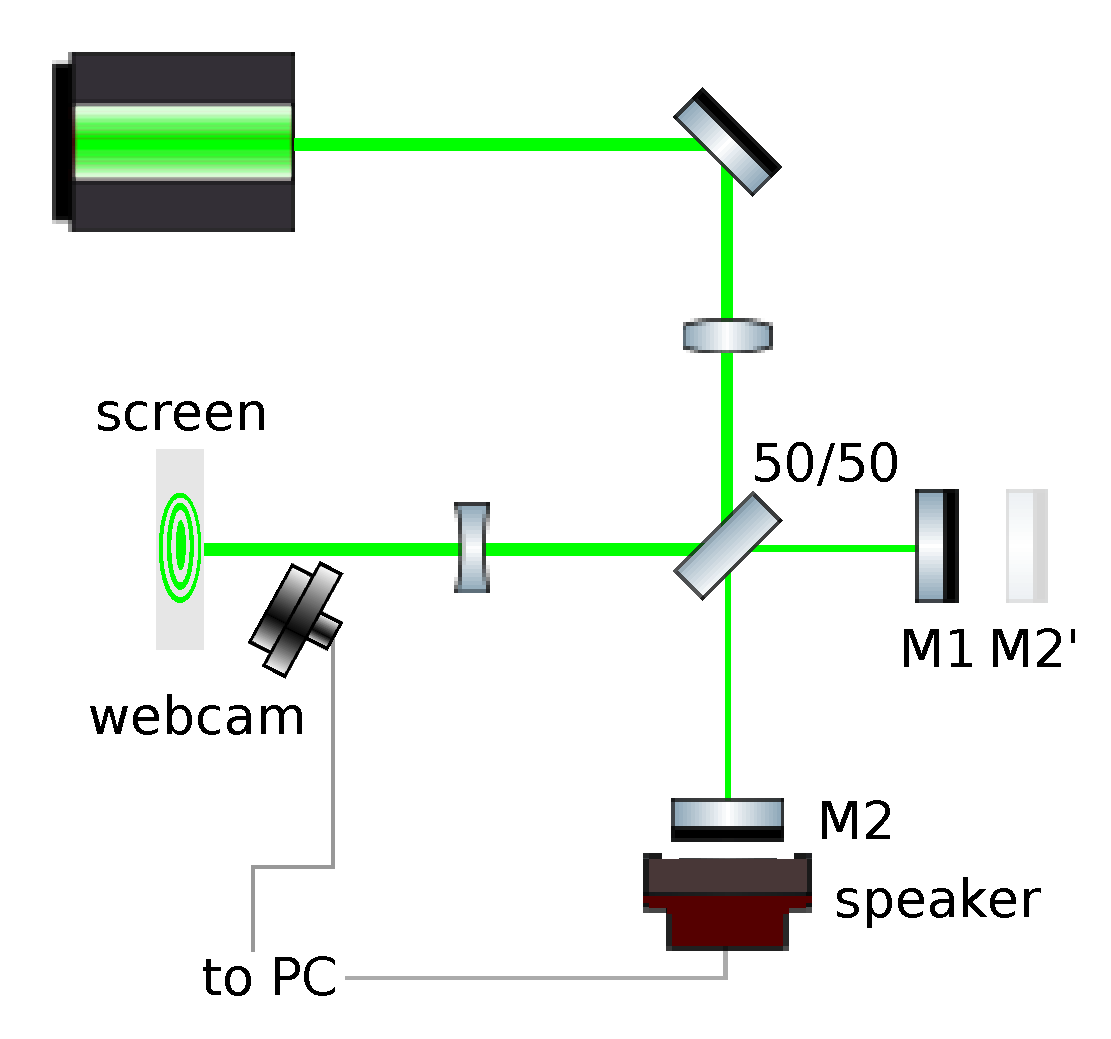
\includegraphics[width=0.8\textwidth]{figures/ifo_schematic_webcam.pdf}
	\caption{Michelson interferometer schematic with interference pattern recorded by a commercial webcam. We used a Class 2 532nm laser~\cite{ThorLabsIFO} and a commercial speaker. The beam is focused at a converging lens before the 50/50 beamsplitter and the interference pattern is made visible by a diverging lens after the beamsplitter. The arms lengths between the speakers are roughly 3cm different and the entire interferometer (without the screen) fits within the dimensions of an A4 piece of paper. We did not include a compensating plate with the beamsplitter, as is often done.}
	\label{fig:ifo_schematic_webcam}
\end{figure}


We used a 0.5W speaker stuck to the back of one of the mirrors as an audio source for our demonstration. This speaker was part of a commercial 3.5mm-jack, USB powered pair of speakers and was driven by a PC. To attach the speaker to one of the mirrors, we wedged it into part of the mirror mount and used commercial adhesive putty to keep it in place. We kept the other speaker in the pair face-down and as far away from the experiment as the cables would allow to reduce it acting as a second source.

As the speaker deforms to play sound, the mirror moves with a change in separation as some coupling function of the amplitude and frequency of the sound. The motion of the fringes follows this motion of the mirror and therefore the speaker at the same frequency.
If the fringe motion is small, then changes in the intensity at some point on the screen follow the frequency of the injected audio but with amplitude given by a transfer function that accounts for the coupling and resonance of the speaker-mirror system.
If the fringe motion was large enough for multiple fringes to pass over the measured point in a single speaker deformation, then over-counting would artificially raise the measured frequency. As such, any motion of the fringes must be kept small by playing sound softly through the speaker.

For later sections, we derive the non-linear relation between the separation of the mirrors and the intensity of the pattern at some point on the screen, this can be found in Appendix~\ref{app:intensity_derivation}.

% Note that we do not include the common compensating plate that equalises the amount of time spent in glass for each beam. We did not find it necessary to include it to be able to demonstrate the results desired.

\begin{figure}[h]
	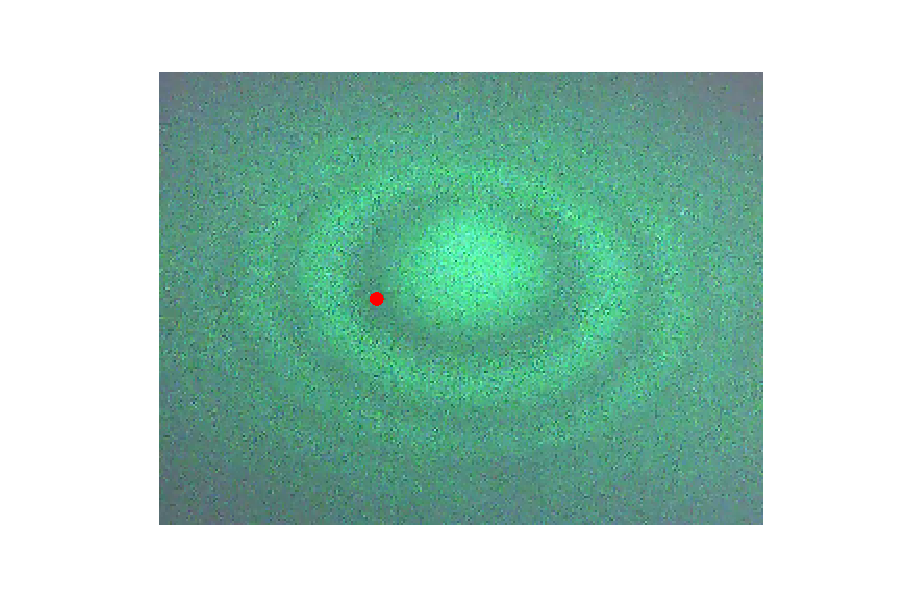
\includegraphics[width=\textwidth]{figures/webcam_still0.pdf}
	\caption{Interference pattern from Michelson interferometer as viewed by webcam from off-centre (hence why the pattern appears non-circular), red dot indicates point where intensity time series was measured from. For scale, the central fringe is approximately 5mm across}
	\label{fig:interference_pattern}
\end{figure}

% A note that while the interference pattern appears similar to the Airy pattern produced by a circular aperture, they are not in fact the same geometry.

    
\section{Observing a wandering tone}
\label{sec:viterbi_wandering}
% Tracking tones with the Viterbi algorithm
% explaination and successful application
% lean on the continuous gravitational waves angle

As also mentioned in Section~\ref{sec:introduction}, continuous wave searches often look for signals that wander slowly in frequency~\cite{2019PhRvD.100l2002A}. The audio analogue of this is a tone that wanders in frequency; a note that changes pitch. Unlike the above Section~\ref{sec:single_tone} though, finding the signal isn’t as simple as searching for a peak in the spectrum for the full observing run.

One method (among many) for continuous wave searches is to split the observed signal into intervals of time, compute the Fourier transform for each time interval, and then create a grid (known as a spectrogram) where each cell is the Fourier amplitude of a particular frequency at a particular time.
This method turns the problem into finding the best path through the spectrogram grid as if it were a weighted graph, where here the weights are the Fourier amplitudes.

When finding the path, the method requires a limit for the allowed frequency change over time, usually informed by a physical model. Here, this frequency wander limit was set to 0.11 Hz per second to make it simply one frequency bin per every time bin, which will prove poorly adjusted to the signal.


\subsection{The Viterbi algorithm}

The Viterbi algorithm is a path-finding algorithm that is used in continuous wave searches~\cite{viterbi_application} to solve this problem.
Abstractly speaking, the algorithm is given a weighted graph (e.g.\ the spectrogram grid), a sensible sequence of subgraphs (e.g.\ the columns of the spectrum at each time), and restrictions on connectivity (e.g.\ the allowed amount frequency wander). Then, at each iteration, it will find the best path to each node in the next subgraph, all the way from the first subgraph. At the end, it selects the overall best path from the first to the last subgraph (here, from the start to end time), this overall best path is called the Viterbi path. See Appendix~\ref{app:viterbi} for the full details of the algorithm in this particular implementation.

\subsection{Results}

We demonstrate this method of using the Viterbi algorithm by injecting a wandering frequency signal into the speaker and recording the output via the webcam.
Note that when creating a wandering frequency signal, the phase change must be integrated up over time, as detailed in Appendix~\ref{app:phase_gotcha}.

\begin{figure}[h]
	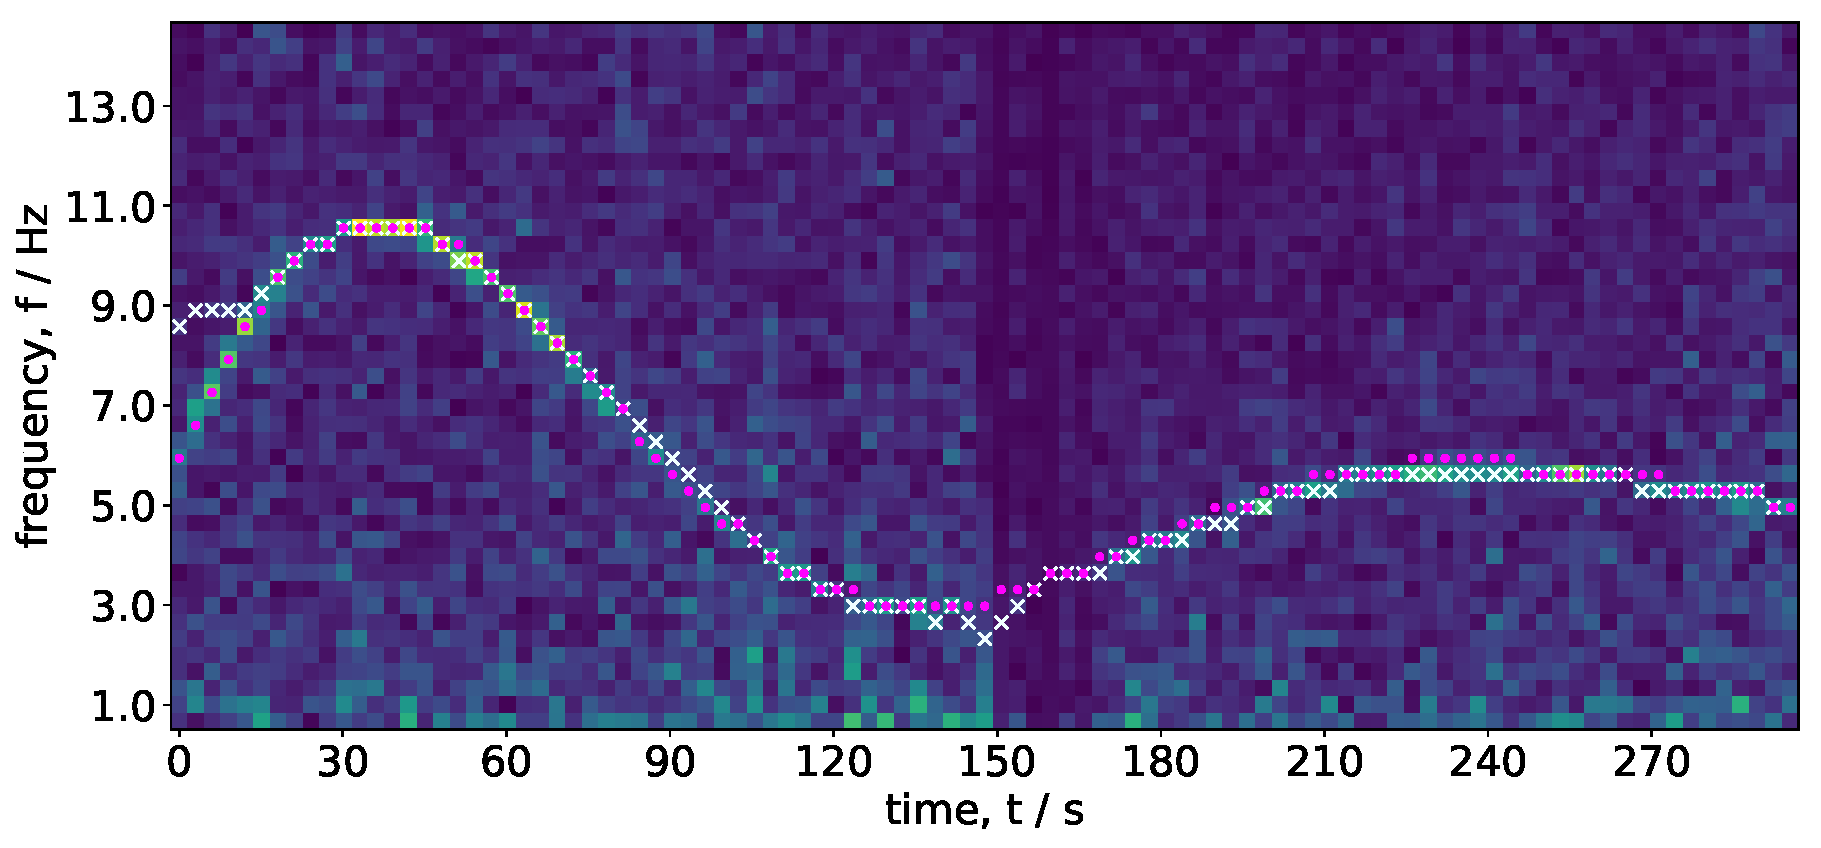
\includegraphics[width=\textwidth]{figures/expt_overlay_2_viterbi_test_webcam.pdf}
	\caption{Spectrogram of observed signal overlaid with pink dots for the injected signal and white crosses for the Viterbi path. Note the high correlation between them. Also note the deviations at the start time when the signal moves too quickly and just before the background anomaly at 150s.}
	\label{fig:viterbi_overlay}
\end{figure}

Shown in Figure~\ref{fig:viterbi_overlay} is the resultant spectrogram of the observed signal, overlaid with the injected signal (the pink dots) and the recovered Viterbi path (the white crosses).
To the eye, the Viterbi algorithm easily recovers the injected frequency over time due to the high signal-to-noise ratio (SNR) of this experiment. Quantifying this, the Viterbi path stays within one frequency bin (approximately 0.3Hz) of the injected tone for 94\% of the run.
Note that the signal initially moves faster than the frequency wander limit, causing a discrepancy between the injected and recovered signals. To fix this, the limit should be doubled, although this would then cause the recovered path to stray more often. There also appears to be an anomaly at 150s, likely from a disturbance (such as someone walking) around the interferometer.

Empirically, decreasing the signal-to-noise ratio closer to unity (by making the speaker quieter) causes the Viterbi algorithm to stray more from the signal. However, since the only correlation through the grid is the signal, we always expect the Viterbi path to lie near to the signal no matter how high the noise is, and this is indeed what we see.

\section{Playing back complex audio}
\label{sec:optical_microphone}
% Optical microphone
% aim of optical microphone: play back injected sounds

The natural succession to observing simple tones is to study complex audio signals, such as music and speech.
The Viterbi algorithm and tracking more broadly is not applicable to these signals. Compare a single tone that slowly, continuously changes frequency to music and speech which consist of a broad spectrum that is constantly changing.
Rather than track them, the interest here is in being able to record and play-back these complex audio signals. Using the interferometer to do so makes it an ‘optical microphone’, using light to capture sound. This device has precedence in the laser microphones~\cite{laser_microphone} of the defence industry which operate on a variety of related principles.


Although this is indirectly related to the advanced signal processing required to extract gravitational wave signals, using an interferometer to capture sound can serve as an interesting demonstration to a broader physics and engineering audience. As such this could be introduced as a separate demonstration.

\subsection{The photodiode method}
\label{sec:photodiode}
% advanced method: explain how we capture data

For the optical microphone to be sensitive to speech and music it needs a frequency response (a sampling rate) far higher than the 30Hz of the webcam. In the context of audible frequencies (roughly 20Hz to 20kHz), speech intelligibility requires frequencies up to 3kHz and music requires frequencies up to and beyond 8kHz~\cite{speech_intelligibility}. Therefore the sampling rate of the optical microphone must be at least 16kHz to capture both speech and music. We achieved this with a photodiode.


A photodiode is an electrical component that acts as a regular diode, blocking any current flow in the `reverse' direction, when no light is incident on it. But as the intensity of incident light rises, it becomes increasingly conductive in the reverse direction. 
% Fundamentally, a current is created in the photodiode by the photo-electric effect.

We placed a (OSRAM BPW21) photodiode in reverse-bias over an (LM358) op-amp to create a photo-detector that would produce a voltage dependent on the incident intensity. We placed the photodiode in the interference pattern at roughly the same off-centre spot as the webcam was monitoring previously (although we saw no difference when monitoring at other positions). The photodiode was mounted on a cloth screen re-purposed from the dismantled commercial speaker, with the electrical leads connected underneath.


The voltage signal from the photo-detector was captured by a (MCP3008) 10-bit analog-to-digital converter (ADC) connected to a Raspberry Pi Model 3 v1.2. Together, these sampled the signal at roughly 16kHz, our desired limit.

However, by sampling, any frequency component of the analog signal above the Nyquist frequency of 8kHz would have been aliased down into the detected range.
To prevent this, we included an anti-aliasing Sallen-Key filter~\cite{sallen_key_filter} tuned to 16kHz before the ADC. This component attenuated any frequencies above 8kHz, before they got digitally sampled. We also had to place another cloth screen over the face of the photodiode, as the reading without it, after gaining through the op-amps, was too high for the ADC.
% It’s not clear what limited the sample rate to 16kHz, but it was likely non-optimal reading of the ADC by the Pi script.
% The ADC used (MCP3008) is quoted at 200kHz (or ksps, kilo samples per second).

A diagram and a photo of the circuit are shown in Appendix~\ref{app:circuit_diagram}. The updated schematic is shown in Figure~\ref{fig:ifo_schematic_podo} and a picture taken of the entire optical microphone is shown in Figure~\ref{fig:setup_pic2}.

\begin{figure}
	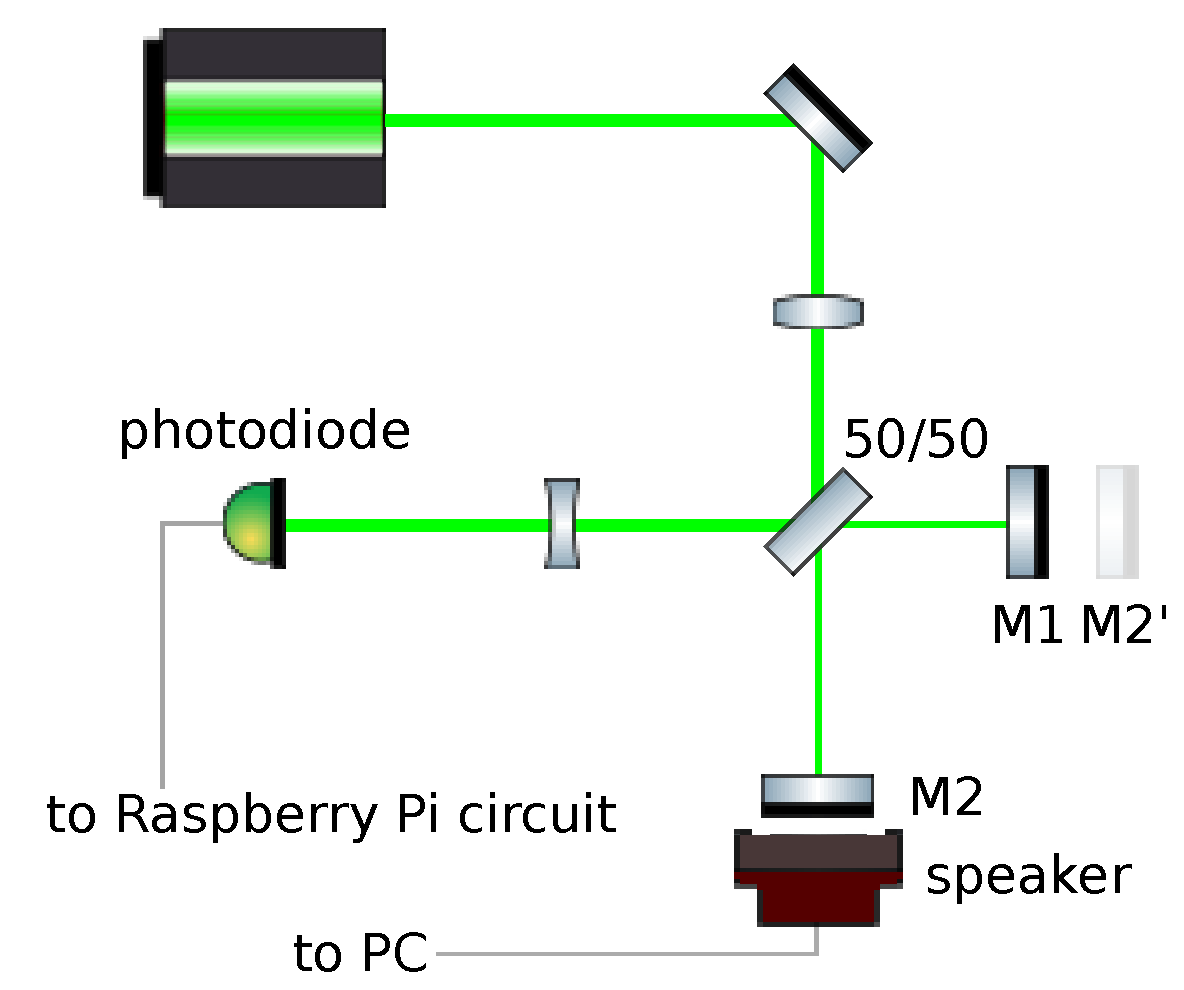
\includegraphics[width=0.8\textwidth]{figures/ifo_schematic_photodiode.pdf}
	\caption{Michelson interferometer schematic with the intensity of the interference pattern at a point measured by a photodiode. See Figure~\ref{fig:ifo_schematic_webcam} for details on the optics configuration.}
	\label{fig:ifo_schematic_podo}
\end{figure}

\begin{figure}
	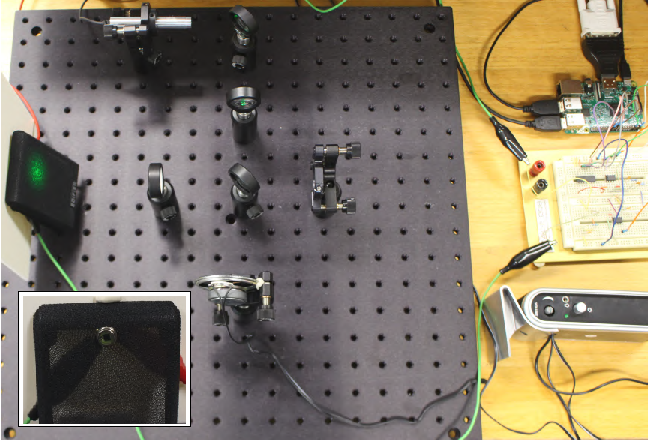
\includegraphics[width=\textwidth]{figures/setup_pic2.pdf}
	\caption{Picture taken of the optical microphone set-up. Showing the Michelson interferometer, the photodiode (behind the cloth screen and in an insert), the circuit, and the Raspberry Pi. See Appendix~\ref{app:circuit_diagram} for a diagram and closer photo of the circuit.}
	\label{fig:setup_pic2}
\end{figure}

\subsection{Initial results of the optical microphone}
% breakdown of all the filters used along the way

The optical microphone was tested on varied recordings of speech from different people and on music ranging from simple melodies to full track songs. Each recording was around one minute long with processing done on ten second segments. For each observation, the audio was played through the speaker as the Pi script recorded the signal from the photodiode. Care was taken to have minimal activity around interferometer while this was happening.
The time series was then directly converted to a .wav file and played as an audio recording, using the \textbf{io.wavfile.write} function from the Scipy~\cite{scipy} package in Python~\cite{python} as before.


When played back, these initial recordings were extremely noisy and had a loud bass hum throughout. Each Fourier spectrum showed dominant AC mains noise with power ranging from the fundamental of 50Hz up to and beyond the 8th harmonic thereof.
With the speaker off this mains power was still present, as shown the power spectral density (effectively the norm squared of the Fourier spectrum) in Figure~\ref{fig:psd_noise}.
And even with the speaker off and the photodiode in complete darkness, the mains hum was still present (with distribution similar to but weaker than that shown in Figure~\ref{fig:psd_noise}).

\begin{figure}[h]%[H]
	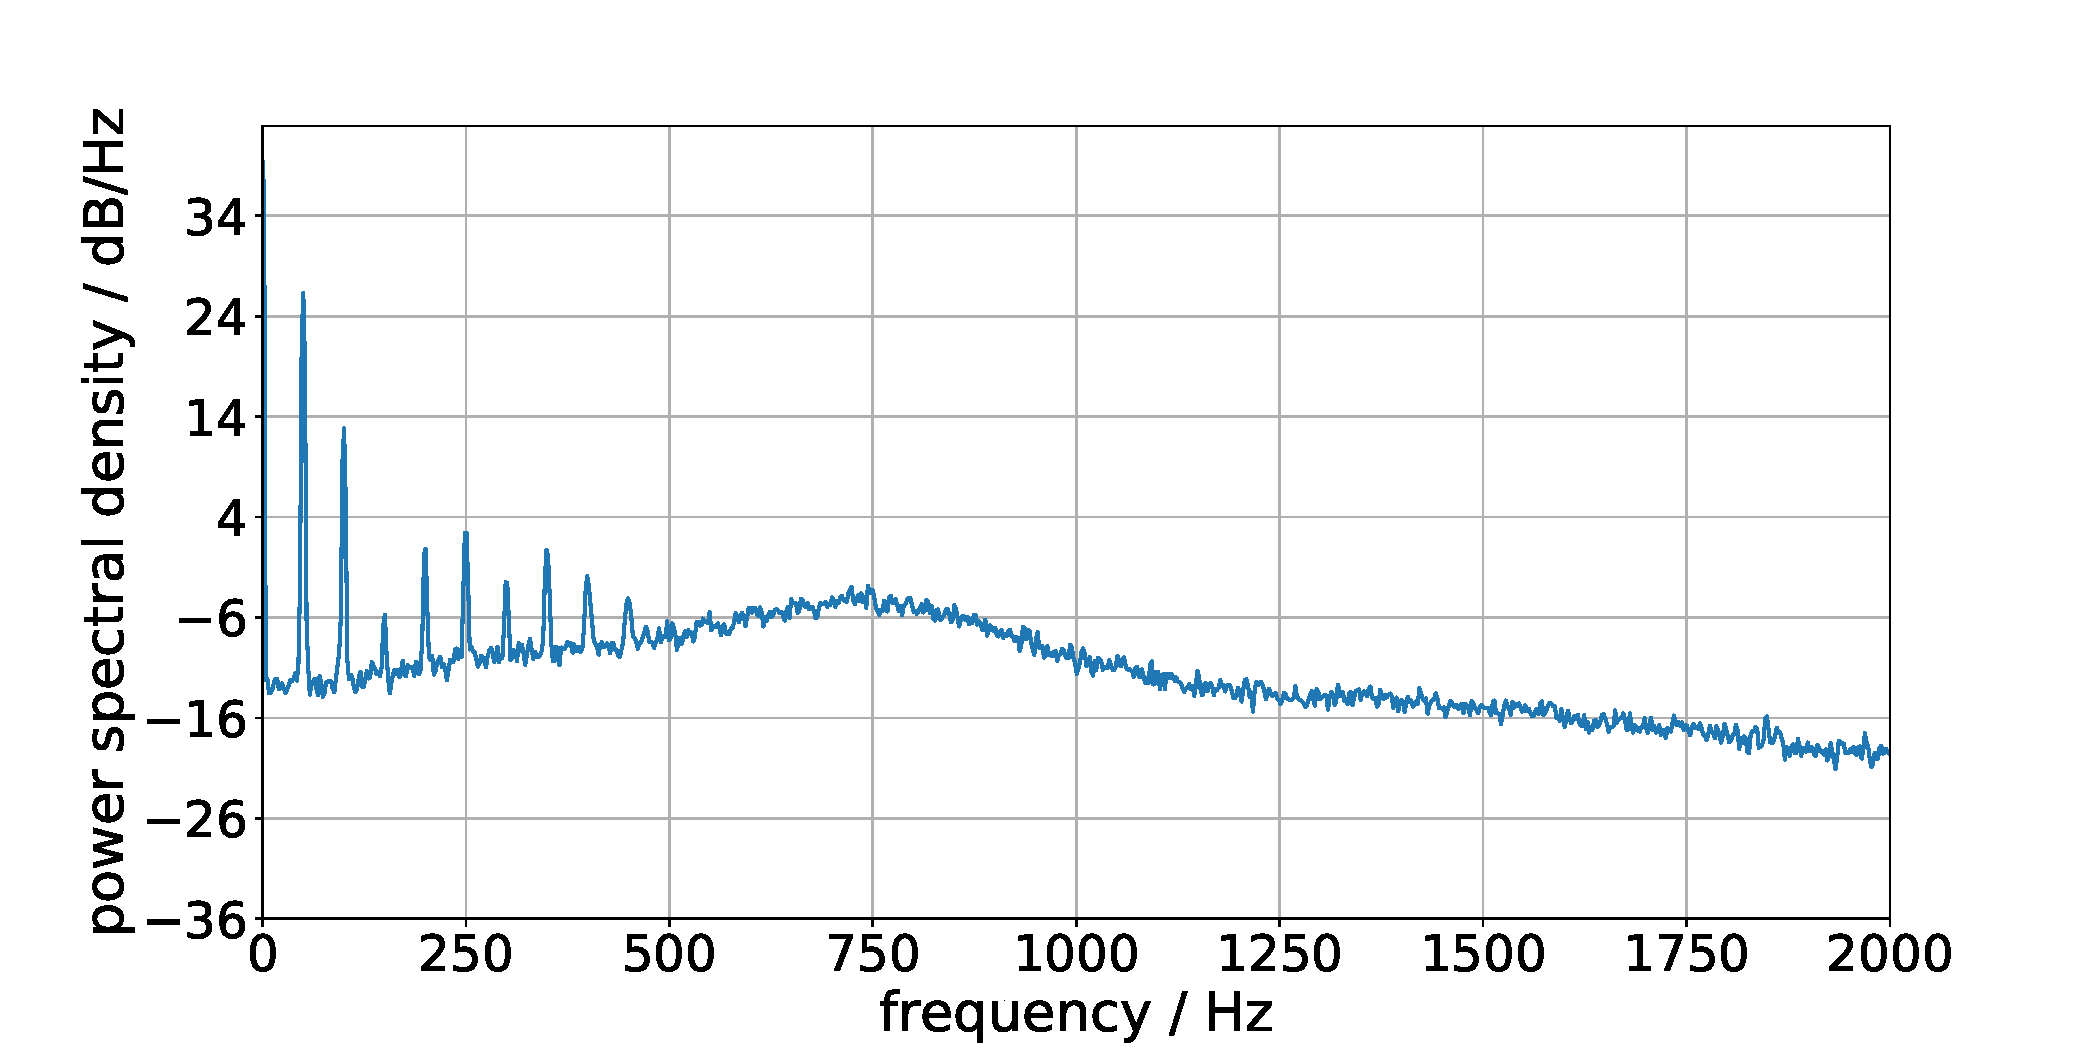
\includegraphics[width=\textwidth]{figures/podo_noise_psd_zoom-cropped.pdf}
	\caption{Power spectral density (PSD) of the optical microphone system with no injected audio (i.e.\ with the speaker off), shows strong power in the 50Hz mains hum and its harmonics (most likely from the photodiode circuit and the surrounding room’s lighting and even cooling), but otherwise is a fairly white spectrum.}
	% except for the broad, shallow maximum at 750Hz}
	\label{fig:psd_noise}
\end{figure}

\subsection{Applying filters to the data}
\label{sec:simple_filters}

The first attempt made to remove the mains hum was to zero the channel of each 50Hz harmonic in the Fourier spectrum. Effectively, this multiplied the spectrum by a rectangular comb filter. While this did remove the mains harmonics, it also audibly ruined the rest of the signal.
This is because applying a filter in frequency space is equivalent to convolving the signal with the inverse Fourier transform of that filter. And the inverse Fourier transform of a rectangular comb filter (a set of boxcars) is a complicated sinc-like function that when convolved with significantly damages the signal.

To fix this, we tried using a smoother comb filter but this too significantly attenuated the rest of the spectrum between each harmonic to hear the signal at all.


Applying a high-pass filter with cut-off frequency 150Hz to the signal worked well at removing the 50Hz and 100Hz tones but was problematic as the mains harmonics extend far past 100Hz and so remain after filtering. This region above 100Hz carries a lot of the fundamental frequencies for speech and music~\cite{speech_intelligibility} and if the cut-off frequency is placed as to remove more of the mains harmonics, then the resultant signal is unrecognisable.

We also tried applying a high-pass filter to the logarithm of the signal spectrum and then exponentiating back, but this didn’t significantly improve on the above simple high-pass.


\begin{figure}[h]%[H]
	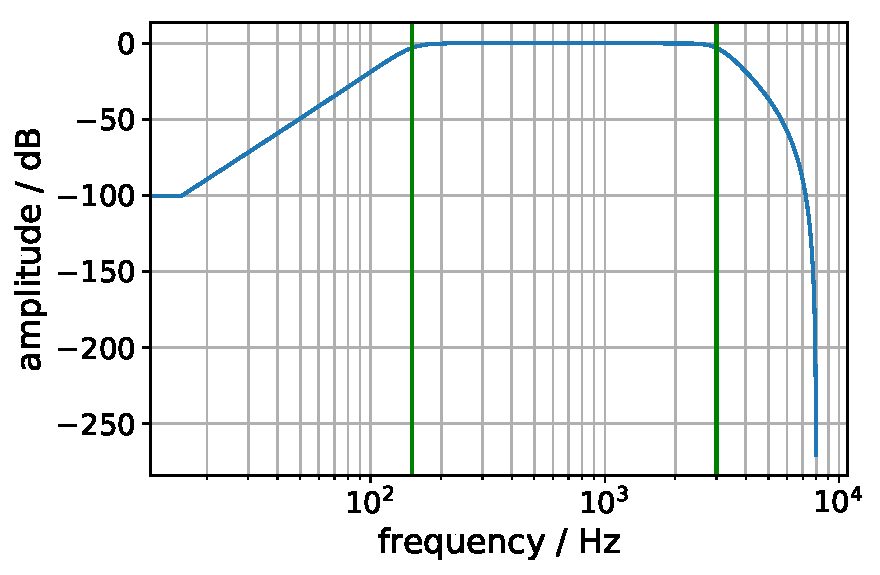
\includegraphics[width=0.8\textwidth]{figures/butterworth_150_3000-cropped.pdf}
	\caption{Butterworth bandpass filter frequency response, any amplitude beyond -3dB is significant attenuation (half power). The green vertical lines show the band limits of 150Hz and 3kHz. Note the flat response within the band.}
	\label{fig:butterworth}
\end{figure}


Band-passing the signal similarly doesn’t address the remaining harmonics above 100Hz but does low-pass away other noise at higher frequencies. The best performing band-pass filter we found was a fifth order ($n = 5$) Butterworth filter over a band from 150Hz to 3kHz (beyond 2kHz speech information content drops significantly~\cite{speech_intelligibility}). For a low-pass Butterworth filter at cut-off frequency $\omega_c$ and gain $\epsilon$ the frequency response (attenuation at each frequency) follows Equation~\ref{eq:butterworth}.
\begin{equation}
\label{eq:butterworth}
H(\omega) = \frac{1}{\sqrt{1+\epsilon^2 (\frac{\omega}{\omega_c})^{2n}}}
\end{equation}
For a Butterworth band-pass filter, the above low-pass filter is combined with a high-pass filter of similar form. The response of the filter used is shown in Figure~\ref{fig:butterworth}. This filter improved on the above simpler filters but recordings of speech still had very low intelligibility, they could be recognised as speech but not understood.


The ideal filter would be one that completely attenuates the undesired parts of the spectrum, does not change the rest of the spectrum, and has smooth edges as to not damage the signal through convolution. These three conditions are contradictory and any filter must compromise between them. The above simple filters fail at one or more of each of these conditions. The combs ruin the signal and the high-passes do not remove the noise. The Butterworth filter performed the best audibly as it is optimised to be `maximally flat' within the band region, prioritising the second condition.

% Note that we also replicated the Viterbi algorithm results from before with the photodiode, but only with the mains hum removed and high-passing above 100Hz, else the algorithm never selected the signal. Except for being over audible frequencies, there isn’t much difference in the tracking once these filters are applied.


\subsection{The logMMSE estimator}
% logMMSE

Speech enhancement for a noisy channel is a classic problem in signal processing. Hu~\&~Loizou~(2006)~\cite{SubjectiveComparison} compared various methods and found the best performing statistical technique among those at the time to be a logMMSE (alt.\ MMSE-LSA) estimator. This type of estimator is based on work by Ephraim~\&~Malah~(1984)~\cite{Ephraim1984SpeechEU_logMMSE} into speech enhancement by minimising the mean square error (MSE) to the logarithm of the spectral (Fourier) amplitude.
Although this technique historically minimised with respect to the spectral amplitude~\cite{EphraimSpeechEU_MMSE}, throughout speech processing use of the logarithm seems produce better results as perceived by the human ear~\cite{SubjectiveComparison}.


We used an existing implementation~\cite{logmmse} of the logMMSE estimator. Applying this estimator to the optical microphone recordings produced dramatically clean results. The time series (in Figure~\ref{fig:logMMSE_timeseries}) and spectrum (in Figure~\ref{fig:logMMSE_spectrum}) from before and after applying the logMMSE filter are shown. Comparing the before and after spectra in Figure~\ref{fig:logMMSE_spectrum} shows significant attenuation of all mains harmonics as well as a general smoothing of the spectrum.


After applying the estimator, simple chords and drums are heard well in played back music. While more complex melodies are sometimes completely absent. By observation, this is especially true for instruments of certain timbres (harmonic profiles), in particular flutes and violins.
This could be a perceptual effect of listening to the lossy recording, but seems more likely to be a frequency dependence somewhere in the optical microphone system. Speculating, perhaps the amplitude of speaker-mirror oscillations is higher at low frequencies and so instruments like electric bass and drums are louder in the results.


After applying the estimator to speech recordings, intelligibility still remains low with the voice sounding mumbled and indistinct. The estimator removes most of the background noise, but does not clarify the speech.

To address these problems with the recordings we need to determine whether the signals that are audibly missing (the diction in the speech and complex melodies in music) are indeed being transmitted through the optical microphone at all. This requires a better understanding of the system and further improvements to the experiment if true.
% The fringe counting problem of the detector, wherein multiple fringes passing over the array in a single speaker deflection artificially raises the frequency, was noticeable in the speech recordings when compared to the source audio. However, upon comparing injected pure tones, the increase appears to be minimal and inconsistent, at around 5Hz maximum difference. An simple explanation is that the speaker deflections are small compared to manual pressing on the optical table.

\begin{figure}%[H]
	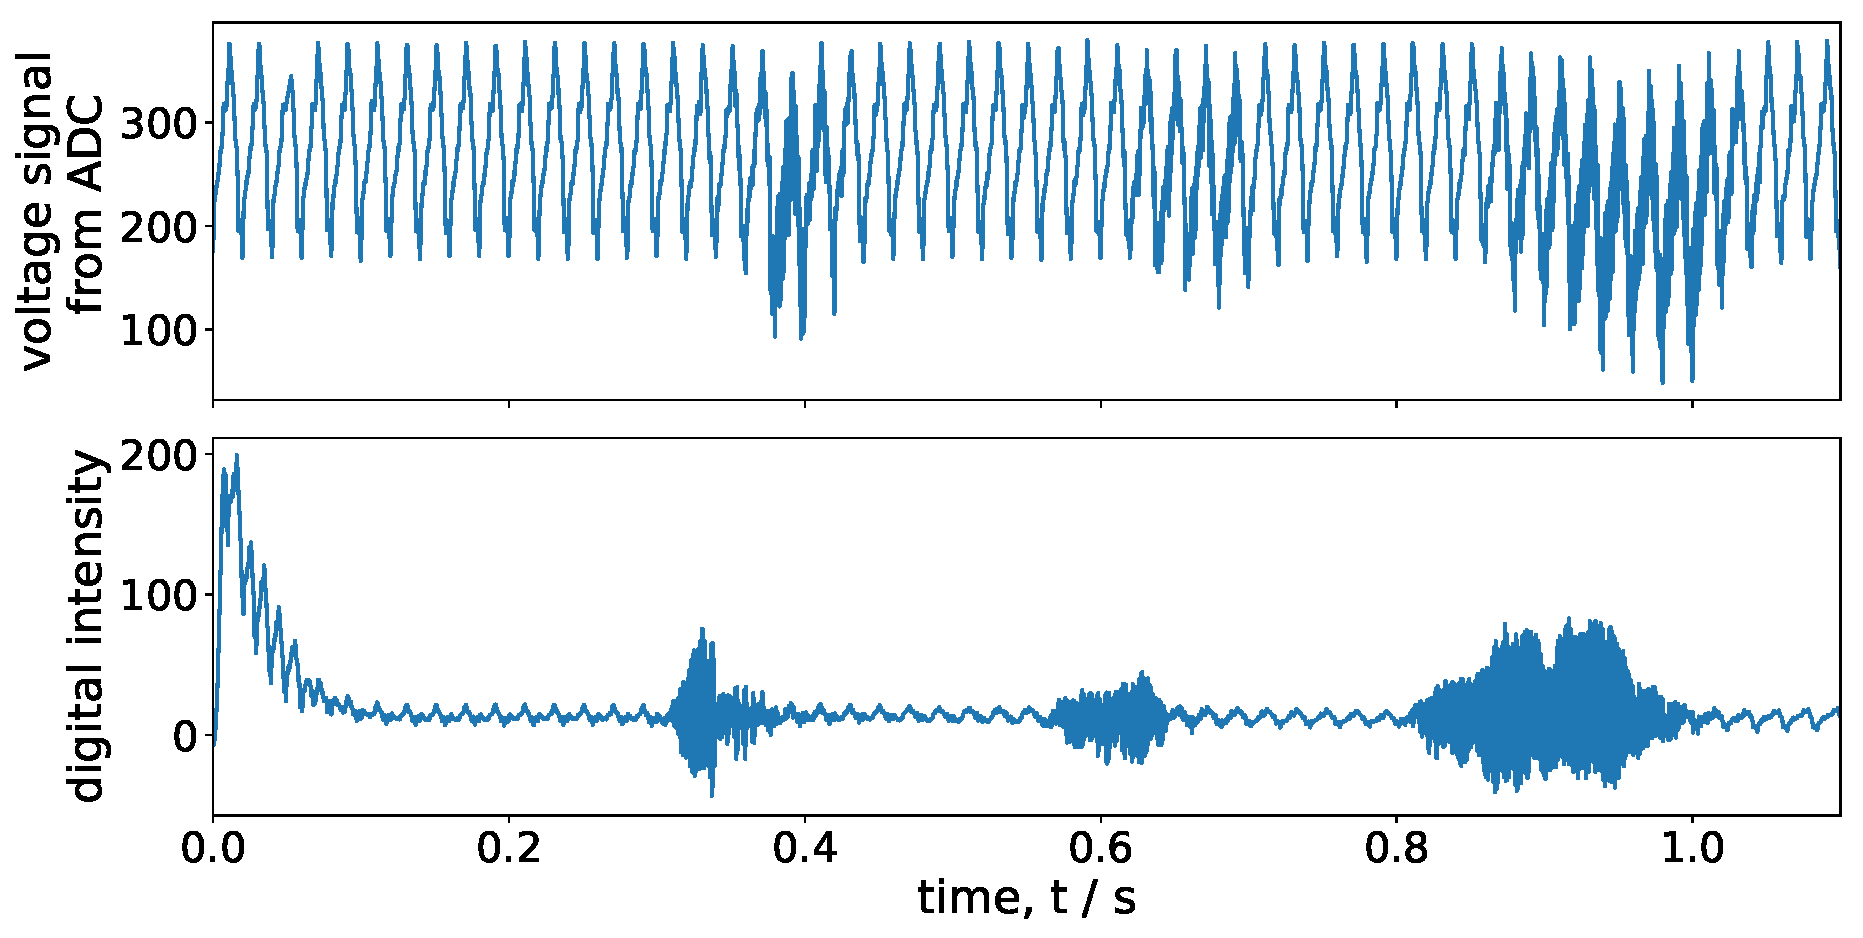
\includegraphics[width=\textwidth]{figures/filter_timeseries_aa_melatos-cropped.pdf}
	\caption{Optical microphone recording of adult male voice (saying ``A cathode ...'') shown before (top) and after (bottom) the logMMSE estimator is applied, showing one second of the one minute recording. The rise at the start of the bottom	 time series is an expected result from filtering a finite signal.}
	\label{fig:logMMSE_timeseries}
\end{figure}

\begin{figure}%[H]
	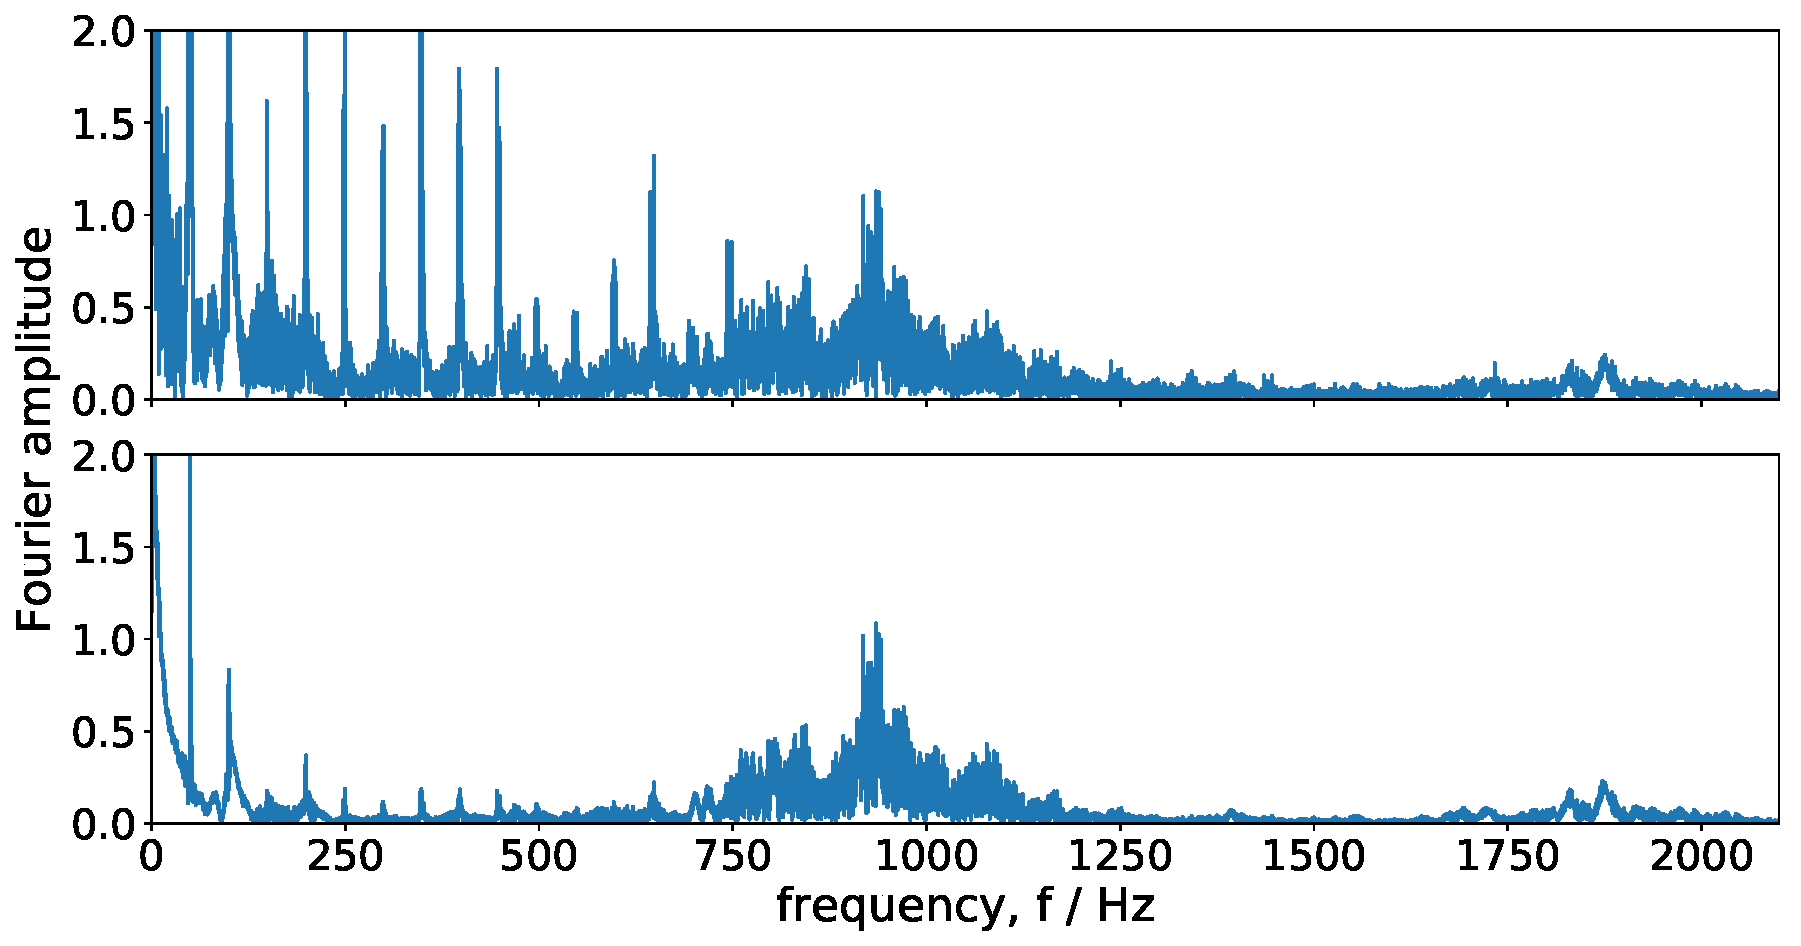
\includegraphics[width=\textwidth]{figures/filter_spectrum_aa_melatos-cropped.pdf}
	\caption{Spectrum of optical microphone recording of adult male voice shown before (top) and after (bottom) the logMMSE estimator is applied, showing only up to 2kHz and to amplitude 2 to see greater detail.}
	\label{fig:logMMSE_spectrum}
\end{figure}


\section{Future work}
\label{sec:future_work}
% wild speculation
We are currently working towards two future advancements for the optical microphone.


The first would be to better isolate the experiment from the mains supply. The Raspberry Pi is USB powered and requires low power so it could even be run off a commercial external phone battery. Everything else in the circuit, including the photodiode, is connected to the Pi, so this would isolate them electrically as well. The laser is DC powered through a converter, so there is no issue there. With the interferometer in a dark room and under a box to better isolate from any ambient light or air currents, this would hopefully remove (or better separate) all sources of the 50Hz mains hum from the optical microphone.


The second advancement would be to achieve a full model of the transfer function of the system. Theoretically, if we had the correct transfer function, then signal recovery would only be limited by the signal-to-noise ratio as we could construct an optimal matched filter. This function would have to start from the voltage sent to the speaker and end with the value recorded by the Pi, and include any non-linearities in the speaker audio production, the speaker-mirror coupling, the separation-intensity relation, and the photodiode reading. This sequence that the signal takes is shown in Figure~\ref{fig:pipeline_highlighted}.


In our investigation, we have currently only derived part of this sequence, the relation between a deflection of the mirror and the change in the intensity of the interference pattern at some point. We find this relation to be non-linear, see Appendix~\ref{app:intensity_derivation} for the derivation.


Asides from the transfer function, for extracting the speech there exists much literature~\cite{HMM_english} on using a hidden Markov model train to English phonemes to recognise speech.
Alternatively, machine learning solutions exist throughout the field that are able to compete~\cite{SEGAN} with statistical techniques like the logMMSE estimator.

To remove the mains hum we could also monitor it separately from the interferometer and subtract the sinusoids with the right phase and amplitude in real (not frequency) space to avoid the problems of Section~\ref{sec:simple_filters}. This could be done with the existing signals if the recording duration is long enough to precisely measure the phase and amplitude over a large number of cycles.


\begin{figure}%[H]
	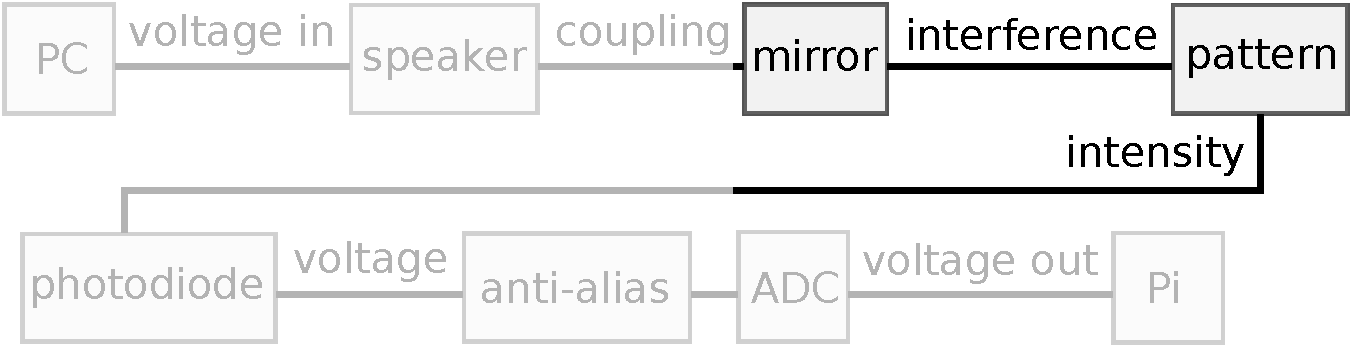
\includegraphics[width=\textwidth]{figures/pipeline_highlighted.pdf}
	\caption{Sequence of relations for optical microphone transfer function. The currently derived relation is highlighted.}
	\label{fig:pipeline_highlighted}
\end{figure}

\newpage
\section{Conclusions}
\label{sec:conclusions}

% Continuous gravitational wave searches use sophisticated statistical techniques to search for weak signals in noisy interferometric data. We demonstrate some of these techniques by observing sound with a table-top Michelson interferometer. In particular, we successfully use the Viterbi algorithm to recover a tone with wandering frequency from a webcam video of the interference pattern.

We use sound and a table-top Michelson interferometer as an analogue to a gravitational wave detector.
% This serves to demonstrate signal processing techniques.


Using a webcam to track the interference pattern, we inject a wandering frequency signal into the system with a speaker attached to the back of one of mirrors of the interferometer. We then demonstrate how to recover this signal using the Viterbi algorithm, just as is done in continuous gravitational wave searches.


Substituting the webcam for the increased frequency response of a photodiode circuit read by a Raspberry Pi, we turned the interferometer into an optical microphone.
We demonstrated that this optical microphone is capable of playing back simple recordings well but that it produces unintelligible recordings of speech. Dominant 50Hz mains hum in the recordings led to an exploration of speech enhancement techniques to remove it, including the well performing logMMSE estimate. From here we have many plans to further remove the mains hum and improve the intelligibility.


These demonstrations have good potential to be adapted into the undergraduate laboratory. There is much to explore in the physics of the interferometer and the astronomy of the motivating continuous gravitational wave searches. Most of all, the signal processing of speech enhancement is an interesting problem that’s relevant to digital communications.


% \bigskip
\newpage
\appendix

\section{Open-source code}
\label{app:code}
This project was implemented in python3~\cite{python} scripts as well as jupyter notebooks~\cite{jupyter}~\cite{ipython} and used the packages of numpy~\cite{numpy}, scipy~\cite{scipy}, matplotlib~\cite{matplotlib}, tqdm~\cite{tqdm}, and logmmse~\cite{logmmse}.

The current build and sample recordings of the optical microphone can be found at:
\url{https://github.com/daccordeon/gravexplain}
% \begin{verbatim}
% README
% \end{verbatim}

\section{Implementation of the Viterbi algorithm}
\label{app:viterbi}

We used the Viterbi algorithm to find a signal in a spectrogram. Here we detail the implementation used.

We consider a spectrogram grid where each element in the grid is the Fourier amplitude of a particular frequency at a particular time. These are normalised between $(0, 1)$ to use as multiplicative weights. In fact, we take the logarithm and so the sum of all weights to avoid underflow. The best path has the highest weight among all paths.

With the grid prepared, the algorithm starts in the second column. In each iteration, the algorithm looks for the best path to each cell from the cells in the previous column, selecting the previous cell with the greatest cumulative weight among those ‘nearby’ (the value of which was discovered in the previous iteration). Where the cumulative weight is the weight of the best path to reach that previous cell. The nearness of a previous cell is given by the limit on the allowed frequency change over time.

For each cell in the current column, the algorithm calculates the cumulative weight to reach that cell by adding its weight to the cumulative weight to reach it. The algorithm also notes the row index of which cell in the previous column it best connects to.
Continuing like this until it reaches the end of the grid, the algorithm then looks for the greatest weight in the last column and retraces the indices of the steps it took until it reaches the start of the grid. That discovered best path is the Viterbi path.


\section{A common mistake for those new to wandering frequency signals}
\label{app:phase_gotcha}

We want to generate a sine wave that changes frequency over time so that the frequency at some time is given by a function $f(t)$. A common mistake is to appeal to the standard form $\sin{(2 \pi f t)}$, where f is a constant frequency, and guess $\sin{(2 \pi f(t) t)}$. However, this fails to address the phase accumulated earlier in the signal. Instead, the standard form in fact says that for some $\sin{(F(t))}$ it is true that $\frac{dF}{dt}(t) = 2 \pi f(t)$, where $f(t)$ gives the frequency of $\sin{(F(t))}$ at time $t$. Therefore, the correct form for a wandering tone is $\sin{(\int{2 \pi f(t) dt})}$.
% This formula is also useful when performing frequency modulation.


\section{Photodiode circuit design}
\label{app:circuit_diagram}
% schematic of breadboard and connections to pi
% https://www.circuit-diagram.org/editor/
% https://crcit.net/c/e397dcc2166943d69155f9dac1e27bce

Figure~\ref{fig:circuit_diagram} shows the photodiode circuit diagram, it is also available at \url{https://crcit.net/c/e397dcc2166943d69155f9dac1e27bce}. A photo of the breadboard and Raspberry Pi pins is shown in Figure~\ref{fig:circuit_pic3}. This design was based off standard examples of photo-detectors, connecting an ADC to a Pi, and Sallen-Key filters.

\begin{figure}[h]%[H]
	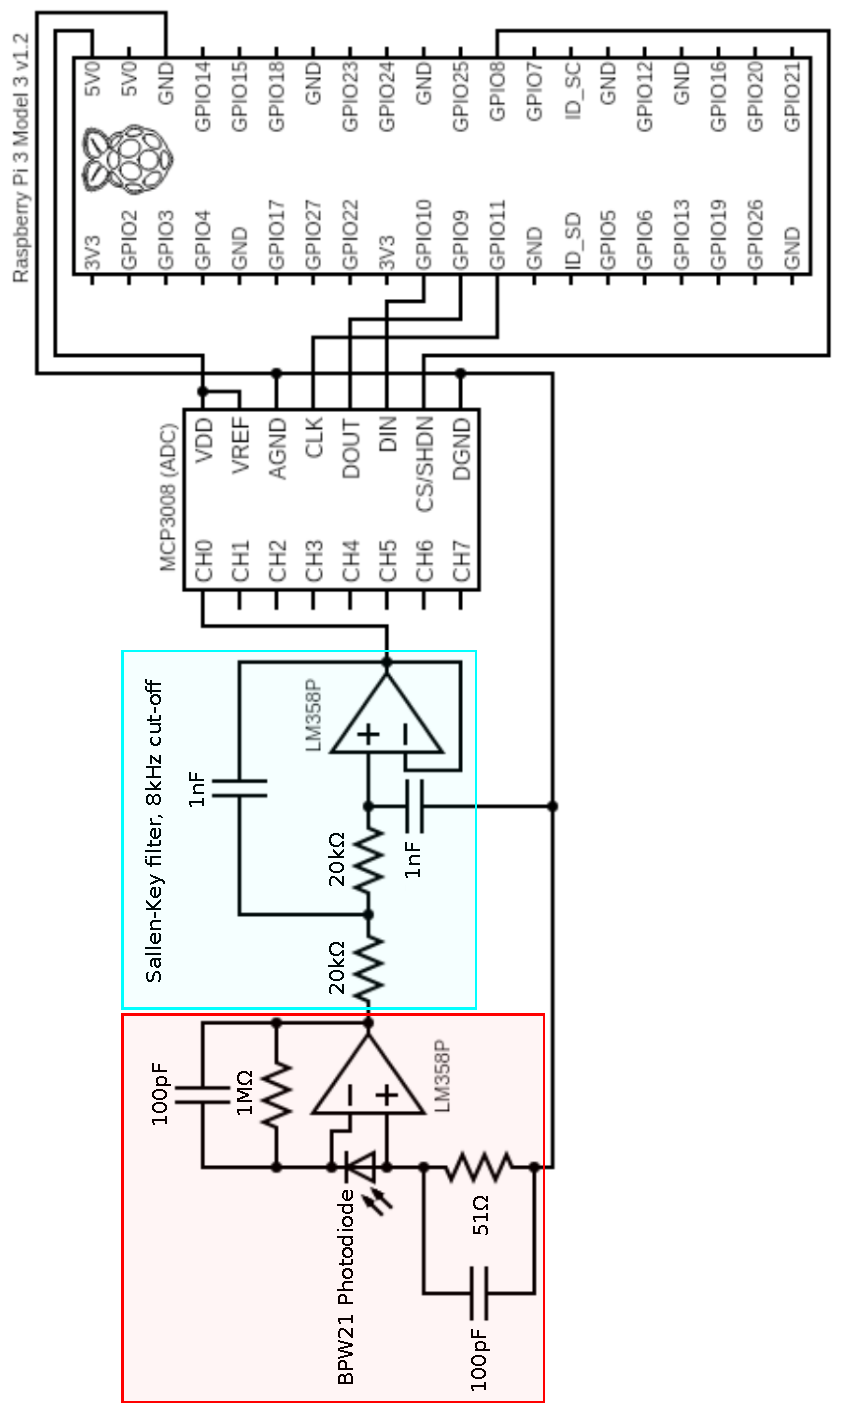
\includegraphics[width=\textwidth]{figures/circuit_diagram_2.pdf}
	\caption{Circuit diagram for photodiode reading. Photodiode in reverse-bias over an op-amp, analog signal then passed through Sallen-Key anti-aliasing filter tuned to 16kHz, then into an analog-to-digital converter (ADC). The digitised signal is then read by the special purpose input (SPI) pins of a Raspberry Pi in standard configuration.}
	\label{fig:circuit_diagram}
\end{figure}

\begin{figure}%[H]
	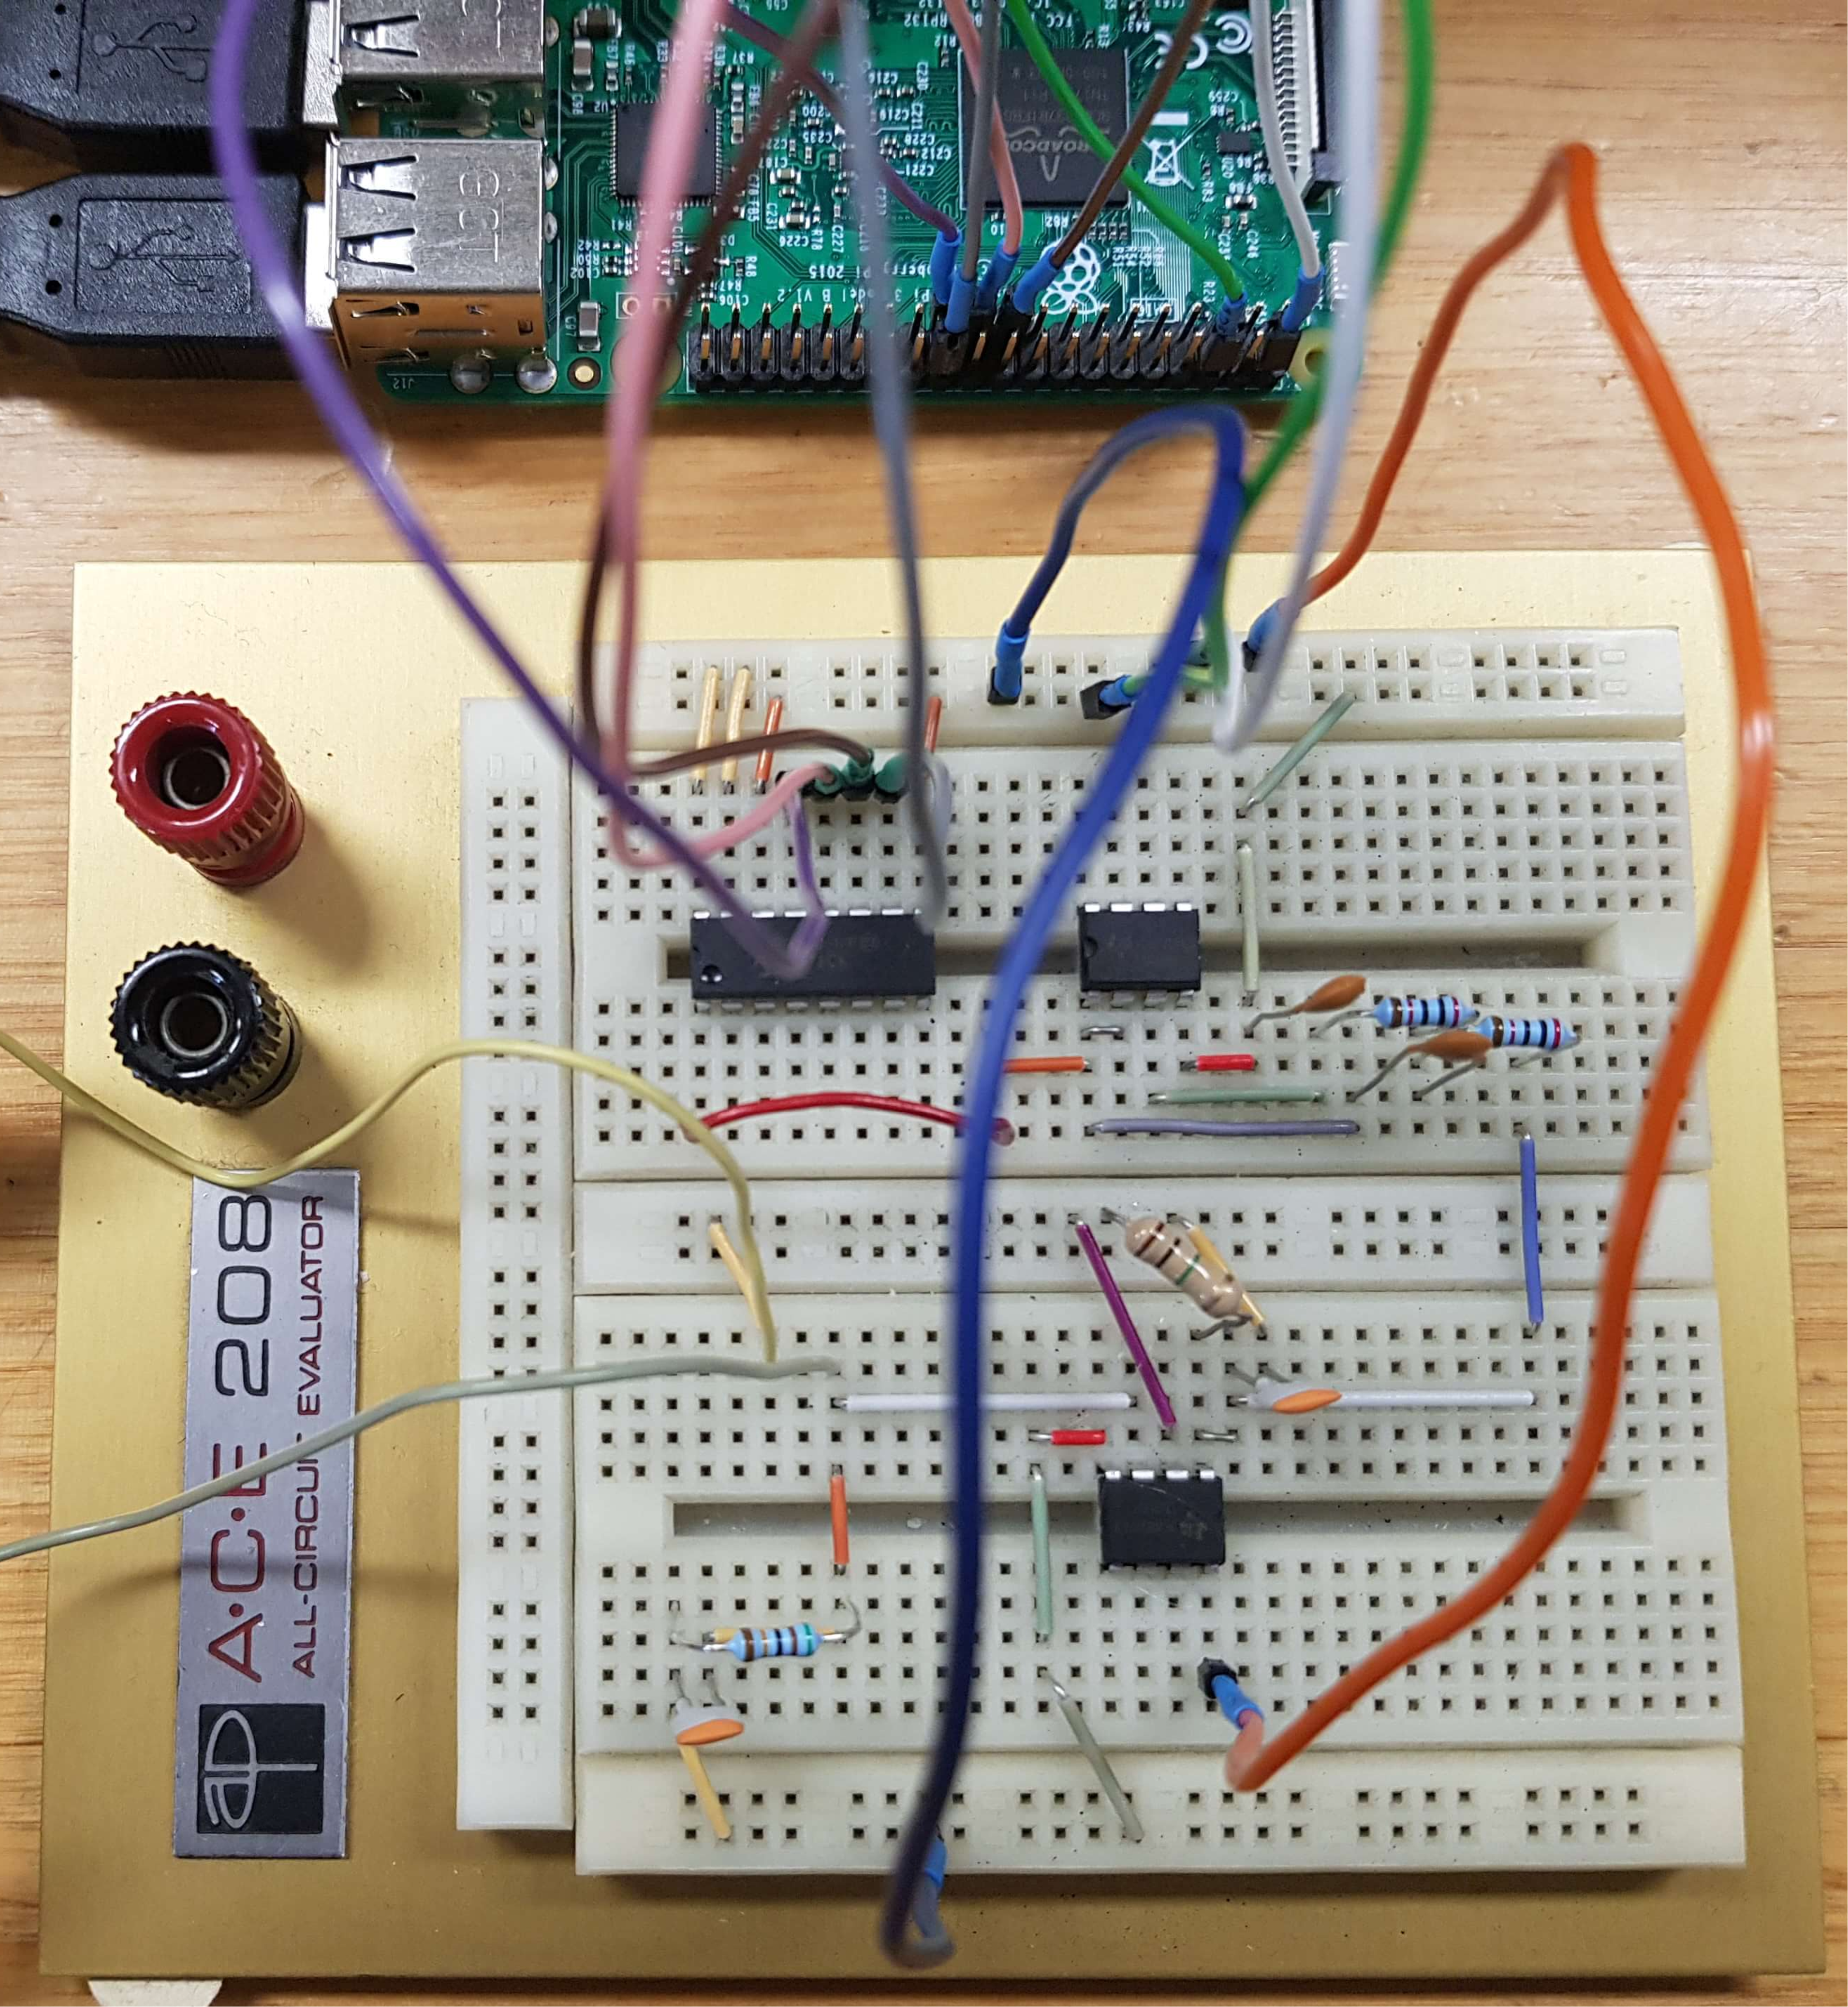
\includegraphics[width=0.8\textwidth]{figures/circuit_pic3.pdf}
	\caption{Photo of photodiode circuit assembled on breadboard.}
	\label{fig:circuit_pic3}
\end{figure}

\section{Interferometric intensity relation derivation}
\label{app:intensity_derivation}

To obtain part of the transfer function for the optical microphone, we want to know the resultant change in intensity, $\delta I$, at a point in the interference pattern, given a small change, $\delta d$, in the difference between the arm lengths of the mirrors. Let the point be at angle $\theta$ on the screen (in the far-field) above the central ray as measured from the mirrors. Noting circular symmetry as to not specify exactly where in the fringe the point is.

At this point, two rays meet, one from each mirror, with total electric field amplitude $E_1(t) + E_2(t)$. Given an initial difference between the arm lengths of $d$, the path difference between the two beams at the screen is $2 d \cos{\theta}$ as the longer beam must travel back and forth over the extra distance, and both travel at angle $\theta$ to meet the point~\cite{fringes:online}.

The intensity at the point is then the norm squared of the total electric field amplitude as expressed in Equation~\ref{eq:intensity_derivation} below.

\begin{align}
    E_1(t) &= A e^{i (k L - \omega t)} \\
    E_2(t) &= A e^{i (k (L + 2 d \cos{\theta}) - \omega t)} \\
    I(t) &= \lvert A e^{i (k L - \omega t)} + A e^{i (k (L + 2 d \cos{\theta}) - \omega t)} \rvert^2
\label{eq:intensity_derivation}    
\end{align}

Collapse the phase difference to some value $\phi = 2 k d \cos{\theta}$. Then expand the norm squared using Euler’s relation, $e^{i \theta} = \cos{\theta} + i \sin{\theta}$. Here we stop considering intensity as a function of time as the time dependence will vanish.

\begin{align}    
    I &= A^2 \lvert e^{i (k L - \omega t)} + e^{i (k L + \phi - \omega t)} \rvert^2,\, \phi = 2 k d \cos{\theta} \\
    I &= A^2 ((\cos{(k L - \omega t)} + \cos{(k L + \phi - \omega t)})^2 + (\sin{(k L - \omega t)} + \sin{(k L + \phi - \omega t)})^2)
\end{align}

Expand and collect like terms, pull out a factor of two, and then recognise the form of $\cos{(\alpha-\beta)}$.

\begin{align}
    I &= A^2 (1 + 2 \cos{(k L - \omega t)} \cos{(k L + \phi - \omega t)} + 1 + 2 \sin{(k L - \omega t)} \sin{(k L + \phi - \omega t)}) \\
    I &= 2 A^2 (1 + \cos{\phi}),\, \phi = \frac{4 \pi d \cos{\theta}}{\lambda}
\end{align}

Finally, changing derivatives and expand $\phi$ to find that the change in intensity given a change in distance is non-linear, that ${\delta I}/{\delta d}$ is non-constant.

\begin{align}    
    \frac{\delta I}{\delta d} &= \frac{\delta I}{\delta \phi}\; \frac{\delta \phi}{\delta d}\\
    \frac{\delta I}{\delta\phi} &= - 2 A^2 \sin{\phi}\\
    \frac{\delta\phi}{\delta d} &= \frac{4 \pi \cos{\theta}}{\lambda}\\
    \therefore \frac{\delta I}{\delta d} &= \frac{- 8 \pi A^2 \cos{\theta}}{\lambda} \sin{(\frac{4 \pi \cos{\theta}}{\lambda} d)}
\end{align}

This non-linearity in part of the transfer function will make the reverse problem of extracting the original signal more difficult.


\begin{acknowledgments}
The authors are grateful to Jude Prezens, Alex Tolotchkoc, and Blake Molyneux for their technical advice and generous assistance throughout the project.
	
The authors are also grateful to Deeksha Beniwal, Sebastian Ng, and Craig Ingram for their advice and work in designing the interferometer. 

This research is supported by the Australian Research Council Centre of Excellence for Gravitational Wave Discovery (OzGrav) (project number CE170100004) and the Institute of Physics International Member Grant.

Travel during the project was supported by the Australian National University PhB Science  program.

\end{acknowledgments}


\bibliographystyle{myunsrt}
\bibliography{ifoDemoBib}

\end{document}

\end{comment}
